%\VignetteIndexEntry{introduction}
\documentclass{article}

%%% latex packages
\usepackage[T1]{fontenc}
\usepackage{hyperref}
\usepackage[utf8]{inputenc}
\usepackage[usenames,dvipsnames]{xcolor}

\usepackage{lipsum} % for dummy text only

%% change margins to 1" all the way around
\oddsidemargin 0.0in
\evensidemargin 0.0in
\textwidth 6.5in
\headheight 0.0in
\topmargin 0.0in
\textheight 9.0in

%%% document info
\title{Introduction to \texttt{SpaDES}}

\author{
  Alex M. Chubaty\\
	\small{Natural Resources Canada, Pacific Forestry Centre}\\
	\small{email: \href{mailto:achubaty@nrcan.gc.ca}{achubaty@nrcan.gc.ca}}
	\and
	Eliot McIntire\\
	\small{Natural Resources Canada, Pacific Forestry Centre}\\
	\small{email: \href{mailto:emcintir@nrcan.gc.ca}{emcintir@nrcan.gc.ca}}
}

\usepackage{Sweave}
\begin{document}
\Sconcordance{concordance:introduction.tex:introduction.Rnw:%
1 31 1 1 0 14 1 1 3 2 0 1 1 1 10 8 0 1 2 7 0 1 5 14 1 1 2 1 0 4 1 1 2 4 %
0 1 2 22 1 1 2 1 0 1 4 2 0 1 2 1 0 3 1 1 5 3 0 1 1 1 2 11 0 1 1 15 0 1 %
7 5 0 1 2 5 0 1 2 7 1}

 % displays code as entered (no arranging lines)

\maketitle

\tableofcontents

\newpage

\section{Spatial Discrete Event Simulation (SpaDES)}
\subsection{Overview}
Why SpaDES exists
\subsection{What is Discrete Event Simulation}

\subsection{SpaDES is a DES}



\newpage

\section{Using SpaDES to build discrete event simulations}
\paragraph{Requirements}
This packages makes heavy use of the \texttt{raster} and \texttt{sp} packages, so familiarity with these packages and their classes and methods is recommended.
\paragraph{}
Talk about doSim and simInit.

\begin{Schunk}
\begin{Sinput}
> times = list(start=0,stop=10.02)
> parameters = list(
+                    .globals=list(mapName="landscape"),
+                    .progress=list(NA),
+                    randomLandscapes = list(nx=1e2, ny=1e2, .saveObjects="landscape",
+                                            .plotInitialTime = 0, .plotInterval=1e3,
+                                            startTime=0),
+                    fireSpread=list(nFires = 1e1, spreadprob=0.225,
+                                    persistprob=0, its=1e6,
+                                    .plotInitialTime = 0.1, .plotInterval=10,
+                                    returnInterval = 10, startTime=0),
+                    caribouMovement=list(N=1e2,
+                                 .plotInitialTime = 1.01, .plotInterval=1,
+                                 moveInterval=1, startTime=0)
+                  )
> modules = list("randomLandscapes", "fireSpread", "caribouMovement")
> path = system.file("sampleModules", package="SpaDES")
> mySim <- simInit(times=times, params=parameters, modules=modules, path=path)
> doSim(mySim)
\end{Sinput}
\end{Schunk}
\includegraphics{introduction-using-SpaDES}

\newpage

\section{SpaDES modules}

\subsection{Module overview}

\paragraph{}
\texttt{SpaDES} modules are event-based, meaning that different actions are performed on data objects based on the order of scheduled events. Basically, a module consists of a collection of events which are scehduled depending on the rules of your simulation. Each event may evaluate or modify a simulation data object, or perform other operations such as saving and loading data objects.

\subsection{Events}

\subsubsection{Simulation event list}
Lorem ipsum ...

\subsubsection{Module events}
Lorem ipsum ...

\subsubsection{Dependencies}
Typically, each module schedules its own events (e.g., a ``fire'' module may schedule ``burn'' events) and only uses its own data objects. Modules that behave in this way are indepedent of each other, and this is generally the prefered way to design and implement modules.

\paragraph{}
For more information about module dependencies please see the \texttt{modules} vignette.

\subsection{Objects}

\subsubsection{Data types}

\paragraph{}
As you build your modules for your simulation, you can use any of \textsf{R}'s data types to store your objects and data. In particular, matrices (including vectors) and lists work well for this purpose because as of \textsf{R} version 3.1 they are more efficient and reduce your model's memory footprint and speeds up your codes execution. Other useful datatypes include \texttt{Raster*} and \texttt{SpatialPoints*} objects.

\subsubsection{Global objects}

\paragraph{}
Use the superassignment operator (\texttt{<}\texttt{<-}) to assign global objects to reduce copying large objects (such as maps), which slows model execution.

\subsubsection{Dependencies}

\paragraph{}
As noted above, modules can depend on one another for event scheduling. Modules can also be design to rely on outputs (data objects) from other modules. A module that relies on a global simulation data object that is also used by another module is said to be dependent on that other module. It is often useful to develop collections of modules that interact indirectly and are dependent on shared data objects.

\paragraph{}
For more information about module dependencies please see the \texttt{modules} vignette.

\newpage

\section{Reading data or maps from files}
There is a function, simLoad, that can use the simList or a fileList directly, to load maps or data from files. This can ease loading of many types of files into R.

\newpage

\section{Simulating ``agents''}

\subsection{Spatial agents}

\subsubsection{Point agents}

\paragraph{}
agents represented by a single set of coordinates indicating their current position.

\paragraph{}
Use a \texttt{SpatialPointsDataFrame} with additional columns as needed.

\paragraph{Non-mobile point agents}
e.g., plants

\paragraph{Mobile point agents}
e.g., animals use a \texttt{SpatialPointsDataFrame}, with additonal columns for agents' previous \texttt{n} positions, and any other columns such as age, sex, group membership, etc.


\paragraph{}
\section{A simple fire model}
\paragraph{Burn some of the forest}
Using the spread function, we can simulate fires, and subsequent changes to the various map layers. Here, spreadProb can be a single probability or a raster map where each pixel has a probability. In the example below, each cell's probability is taken from the Percent Pine map layer.

\begin{Schunk}
\begin{Sinput}
> nFires <- 10 # number of agents
> landscape[["Fires"]] <-
+   spread(landscape[[1]],
+          loci=as.integer(sample(1:ncell(landscape), nFires)),
+          spreadProb=landscape[["percentPine"]]/(maxValue(landscape[["percentPine"]])*5)+0.1,
+          persistance=0,
+          mapFireID=TRUE,
+          mask=NULL,
+          maxSize=1e8,
+          directions=8,
+          iterations=1e6,
+          plot.it=FALSE,
+          mapID=TRUE)
> simPlot(landscape[["Fires"]])
\end{Sinput}
\end{Schunk}


\begin{Schunk}
\begin{Sinput}
> # Show the burning more strongly over abundant pine
> simPlot(landscape[["percentPine"]], col=.cols[[3]])
> simPlot(landscape[["Fires"]], add=TRUE, delete.previous=FALSE, col=.cols[[1]])
\end{Sinput}
\end{Schunk}
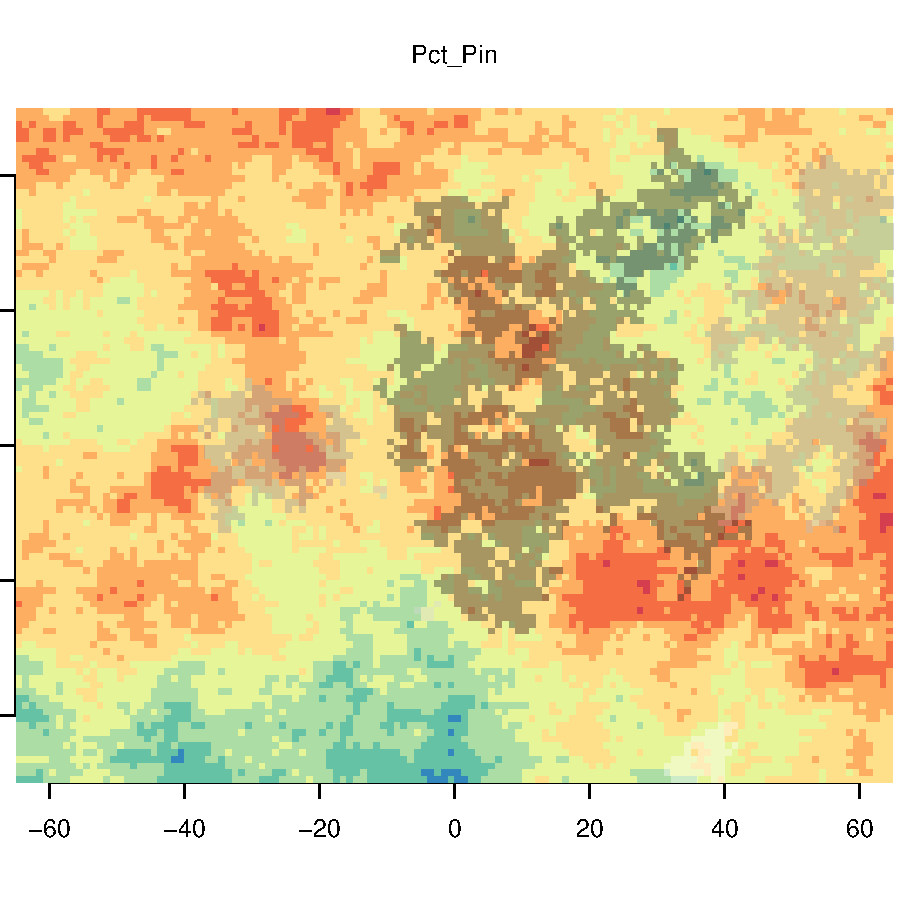
\includegraphics{introduction-fire-overlaid}


\paragraph{}
We can see that the fires tend to be in the Pines because we made it that way, using an arbitrary weighting with pine abundance

\begin{Schunk}
\begin{Sinput}
> # Show the burning more strongly over abundant pine
> fire <- reclassify(landscape[["Fires"]],rcl= cbind(0:1,c(0,ncell(landscape)),0:1))
> pine <- reclassify(landscape[["percentPine"]],rcl= cbind(0:9*10, 1:10*10, 0:9))
> PineByFire <- crosstab(fire, pine, long=TRUE)
> colnames(PineByFire) <- c("fire", "pine", "freq")
> PineByFire$pine <- as.numeric(as.character(PineByFire$pine))
> summary(glm(freq ~ fire*pine, data=PineByFire, family="poisson"))
\end{Sinput}
\begin{Soutput}
Call:
glm(formula = freq ~ fire * pine, family = "poisson", data = PineByFire)

Deviance Residuals: 
    Min       1Q   Median       3Q      Max  
-40.631  -10.346   -2.539    8.542   34.637  

Coefficients:
             Estimate Std. Error z value Pr(>|z|)    
(Intercept)  7.027853   0.018319  383.64   <2e-16 ***
fire1       -3.478185   0.093695  -37.12   <2e-16 ***
pine        -0.050061   0.003674  -13.63   <2e-16 ***
fire1:pine   0.239021   0.014292   16.72   <2e-16 ***
---
Signif. codes:  0 '***' 0.001 '**' 0.01 '*' 0.05 '.' 0.1 ' ' 1

(Dispersion parameter for poisson family taken to be 1)

    Null deviance: 14668.2  on 18  degrees of freedom
Residual deviance:  7326.6  on 15  degrees of freedom
AIC: 7463

Number of Fisher Scoring iterations: 6
\end{Soutput}
\end{Schunk}

\paragraph{}
Sure enough, there are more fires as the abundance of pine goes up, as seen by the positive interaction term (the negative \texttt{fire1} term means that there are more pixels without fires than with fires).

\paragraph{Impact some of the forest}
\begin{Schunk}
\begin{Sinput}
> landscape[["forestAge"]][landscape[["Fires"]]>0] <- 0
> landscape[["forestCover"]][landscape[["Fires"]]>0] <- 0
> landscape[["habitatQuality"]][landscape[["Fires"]]>0] <- 0.1
> landscape[["percentPine"]][landscape[["Fires"]]>0] <- 0
> simPlot(landscape, col=.cols[c(2:5,3,1)])
\end{Sinput}
\end{Schunk}
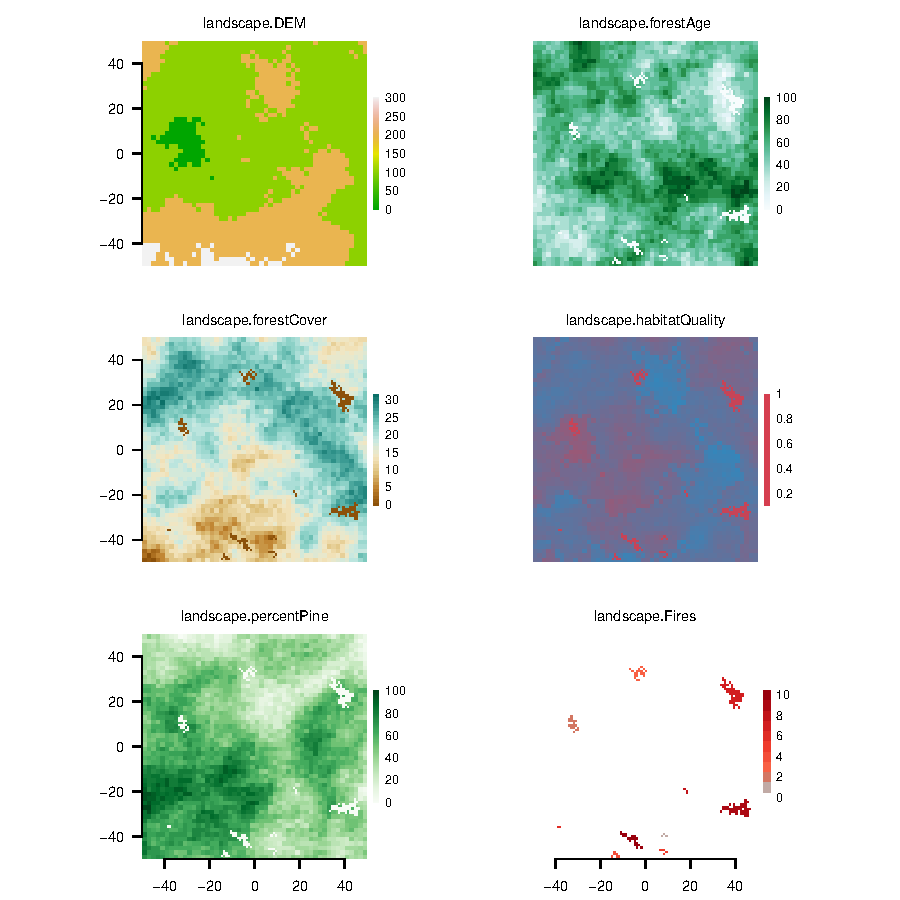
\includegraphics{introduction-fire-impacts-maps}

\section{A simple individual based model (IBM)}
\paragraph{Move some agents}
Using a simple landscape-depedent correlated random walk, simulate the movement of caribou across a heterogeneous landscape. Because we had just had fires, and we assume that fires have a detrimental effect on animal movement, we can see the long steps taken in the new, low quality, post-burn sections of the landscape.

\begin{Schunk}
\begin{Sinput}
> simPlot(landscape[["habitatQuality"]], col=.cols[[3]])
> for (i in 1:10) {
+   #crop any caribou that went off maps
+   caribou <<- crop(caribou,landscape)
+   drawArrows(from=SpatialPoints(cbind(x=caribou$prevX, y=caribou$prevY)),
+              to=caribou,length=0.04,
+              on.which.to.plot=1)
+ 
+   # find out what pixels the individuals are on now
+   ex <- landscape[["habitatQuality"]][caribou]
+ 
+   #step length is a function of current cell's landscape quality
+   sl <- 0.25/ex
+ 
+   ln <- rlnorm(length(ex), sl, 0.02) # log normal step length
+   sd <- 30 # could be specified globally in params
+ 
+   caribou <<- crw(caribou, stepLength=ln, stddev=sd, lonlat=FALSE)
+ }
\end{Sinput}
\end{Schunk}
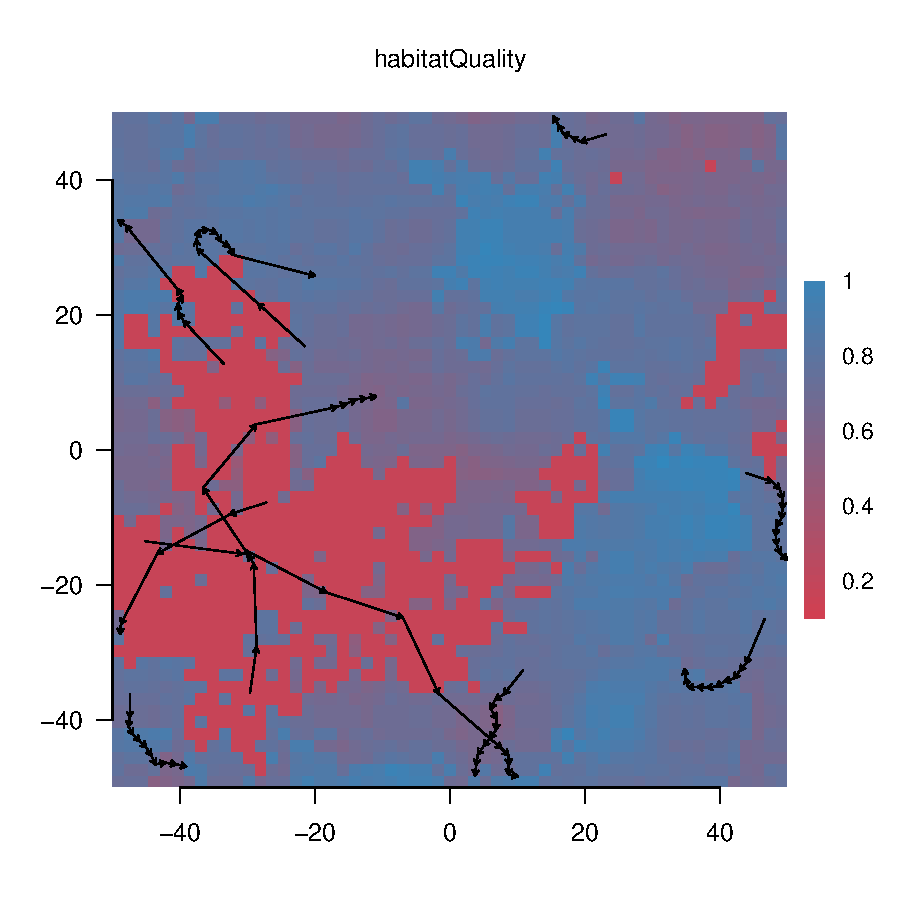
\includegraphics{introduction-agent-crw-trajectory}

\newpage

\section{Further reading}

\subsection{Other \texttt{SpaDES} vignettes:}

%% list all other vignettes here
\begin{itemize}
\item \texttt{modules}: Building modules in \texttt{SpaDES}
\item \texttt{plotting}: Plotting with \texttt{simPlot} in \texttt{SpaDES}
\end{itemize}

\end{document}
